\documentclass[border=10pt]{standalone}
\usepackage{pgf,tikz,pgfplots}
\usetikzlibrary{quotes, angles}
\usetikzlibrary{positioning}
\usetikzlibrary{arrows.meta}
\usetikzlibrary{calc, shapes, automata, fit}
\tikzset{%
	% Specifications for style of nodes:
	base/.style = {rectangle, rounded corners, draw=black,
		%		minimum width=4cm, minimum height=1cm,
		inner sep=15pt,
		text centered, font=\sffamily}, 
	activityStarts/.style = {base, fill=blue!30},
	startstop/.style = {base, fill=red!30},
	activityRuns/.style = {base, fill=red!30},
	process/.style = {base, minimum width=2.5cm, fill=orange!15,
		font=\ttfamily},
	context/.style = {base, inner sep=5pt, align=justify, fill=blue!30}
}
\makeatletter
\tikzset{
	database/.style={
		path picture={
			\draw (0, 1.5*\database@segmentheight) circle [x radius=\database@radius,y radius=\database@aspectratio*\database@radius];
			\draw (-\database@radius, 0.5*\database@segmentheight) arc [start angle=180,end angle=360,x radius=\database@radius, y radius=\database@aspectratio*\database@radius];
			\draw (-\database@radius,-0.5*\database@segmentheight) arc [start angle=180,end angle=360,x radius=\database@radius, y radius=\database@aspectratio*\database@radius];
			\draw (-\database@radius,1.5*\database@segmentheight) -- ++(0,-3*\database@segmentheight) arc [start angle=180,end angle=360,x radius=\database@radius, y radius=\database@aspectratio*\database@radius] -- ++(0,3*\database@segmentheight);
		},
		minimum width=2*\database@radius + \pgflinewidth,
		minimum height=3*\database@segmentheight + 2*\database@aspectratio*\database@radius + \pgflinewidth,
	},
	database segment height/.store in=\database@segmentheight,
	database radius/.store in=\database@radius,
	database aspect ratio/.store in=\database@aspectratio,
	database segment height=0.1cm,
	database radius=0.25cm,
	database aspect ratio=0.35,
}
\makeatother

\begin{document}
%	\path let
%	\p1 = (question),
%	\p2 = (contextEncoder)
%	in
%	coordinate (questionEncoder) at (\x2, \y1);
%	\node (questionEncoder) [rounded corners, fill=orange!50, inner xsep=15pt, inner ysep=10pt, font=\fontsize{14pt}{\baselineskip}\selectfont\sffamily, draw=black] at (questionEncoder) {Question\\ Encoder};
%	\draw[->] (question) -- (questionEncoder);
	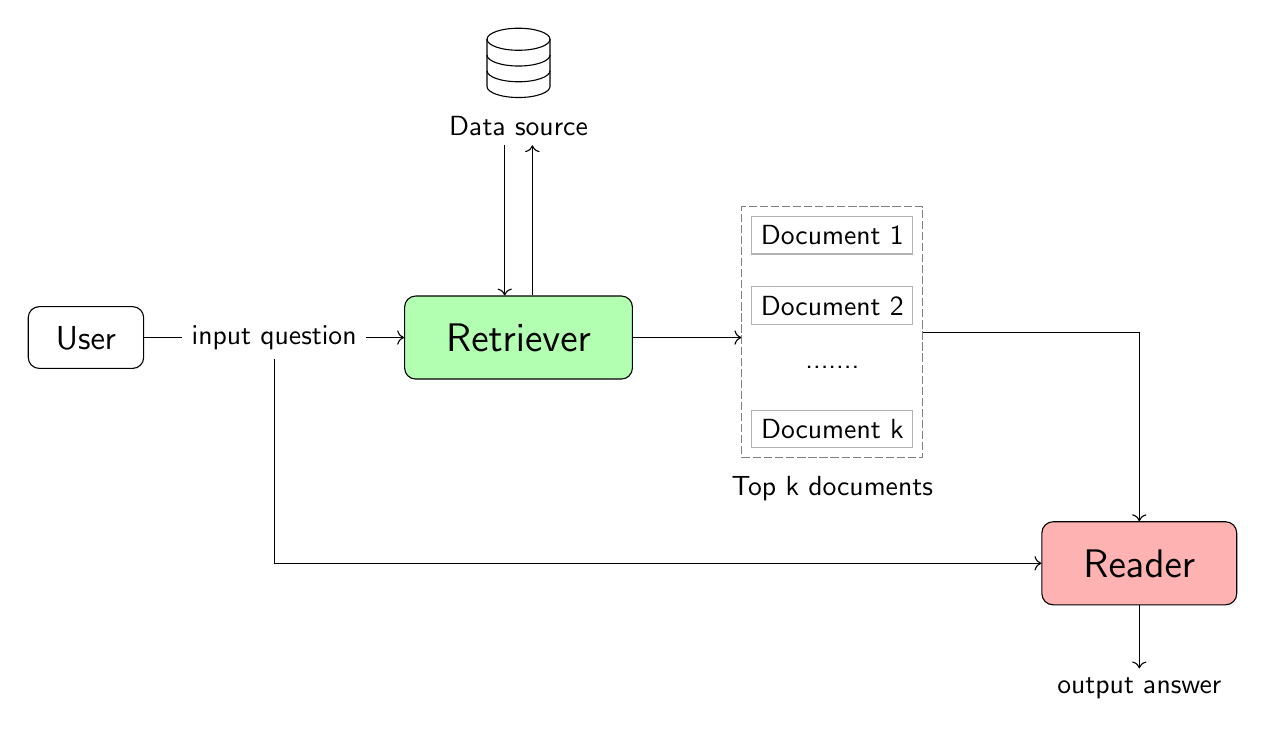
\begin{tikzpicture}[every node/.style={font=\sffamily}, align=center]
		\node (retriever) [rounded corners, fill=green!30, inner xsep=15pt, inner ysep=10pt, font=\fontsize{14pt}{\baselineskip}\selectfont\sffamily, draw=black] {Retriever};
		\node (user) [rounded corners, inner xsep=10pt, inner ysep=7pt, font=\fontsize{12pt}{\baselineskip}\selectfont\sffamily, draw=black, left=3.3cm of retriever] {User};
		\draw[->] (user) -- node (inputQuestion) [fill=white] {input question} (retriever);
		\node (dataSource) [database, database segment height=.2cm, database radius=.4cm, above=2.5cm of retriever] {};
		\node (dataSourceText) [below=0.1cm of dataSource] {Data source};
		\path let
			\p1 = (dataSourceText.south),
			\p2 = (retriever.north)
		in
			coordinate (leftCtxAnchor) at (\x2 - 5pt, \y1);
		\path let
			\p1 = (dataSourceText.south),
			\p2 = (retriever.north)
		in
			coordinate (rightCtxAnchor) at (\x2 + 5pt, \y1);
		\path let
			\p1 = (retriever.north)
		in
			coordinate (retrieverCtxLeftAnchor) at (\x1 - 5pt, \y1);
		\path let
			\p1 = (retriever.north),
		in
			coordinate (retrieverCtxRightAnchor) at (\x1 + 5pt, \y1);
		
		\draw[->] (leftCtxAnchor) -- (retrieverCtxLeftAnchor);
		\draw[->] (retrieverCtxRightAnchor) -- (rightCtxAnchor);
		\node (doc1) [right=1.5cm of retriever, yshift=1.3cm, draw=black!30] {Document 1};
		\node (doc2) [below=.4cm of doc1, draw=black!30] {Document 2};
		\node (docDots) [below=.4cm of doc2] {.......};
		\node (docK) [below=.4cm of docDots, draw=black!30] {Document k};
		\node (topDocs) [fit={(doc1) (docK)}, draw=black!50, dash pattern=on 3pt off 1pt] {};
		\node (topDocsText) [below=.1cm of topDocs] {Top k documents};
		\path let
			\p1 = (retriever.east),
			\p2 = (topDocs.west)
		in
			coordinate (topKVsRetrieverAnchor) at (\x2, \y1);
		\draw[->] (retriever) -- (topKVsRetrieverAnchor);
		\node (reader) [rounded corners, inner xsep=15pt, inner ysep=10pt, font=\fontsize{14pt}{\baselineskip}\selectfont\sffamily, below right=0.8cm and 1.5cm of topDocs, fill=red!30, draw=black] {Reader};
		\draw[->] (inputQuestion.south) |- (reader.west);
		\draw[->] (topDocs) -| (reader);
		\node (answer) [below=.8cm of reader] {output answer};
		\draw[->] (reader) -- (answer);
	\end{tikzpicture}
\end{document}